% chktex-file 44
% chktex-file 36
% chktex-file 13
% chktex-file 1

% =====================================================================
%  Plan4ARI - Deliverable D2.1 (A2 revision)
%  Updated Scientific Plan and First Running Mockup for Low-Code
%  Programming with Generative and Deliberative AI
%
%  Class: ../../latex-style/plan4ari_report.cls (layout of the Plan4ARI D1.1 template)
%  Build: latexmk d21_v1.tex      (XeLaTeX, see latexmkrc)
%  Source: ../Plan4ARI_D2.1_Updated_Scientific_Plan_v0.11.docx
% =====================================================================
\documentclass{plan4ari_report}
\usepackage{tikz}
\usetikzlibrary{arrows.meta,positioning,calc}
\usepackage{amsmath,amssymb}
\usepackage{cite}
\setlength{\emergencystretch}{2em}% slash-joined terms (MI.RA/Dexter, domain/problem) in justified text

\deliverable{D2.1}
\deliverabletitle{Updated Scientific Plan and First Running Mockup for Low-Code Programming with Generative and Deliberative AI}
\docstatusline{Draft~-~Version 0.11}
\inforow{Project acronym}{Plan4ARI}
\inforow{Project duration}{48 months}
\inforow{Work package/activity}{Activity 2~-~Low-code programming exploiting generative and deliberative AI}
\inforow{Task basis}{Task 2.1~-~Update of the scientific plan with the latest state-of-the-art methodologies and tools}
\inforow{Activity / task period}{Activity 2: M1--M36; Task 2.1: M1--M12 (proposed revised specification)}
\inforow{Contractual delivery point}{M12~-~scientific plan and first running mockup}
\inforow{Document status}{Draft for consortium review~-~Version 0.11}
\inforow{Lead beneficiary}{To be confirmed (technical drafting: CNR-STIIMA/Plan4ARI team)}
\inforow{Dissemination level}{RESERVED}
\inforow{Evidence cut-off}{Literature review: 21 July 2026; mockup and submission planning update: 23 September 2026}

\begin{document}
\makecover%

\begin{documentcontrol}
\docversion{0.1}{20 July 2026}{Plan4ARI team}{Initial outline}
\docversion{0.9}{21 July 2026}{Draft prepared for consortium review}{Filled scientific plan; literature update; revised architecture and roadmap}
\docversion{0.10}{23 September 2026}{Draft for consortium review}{M12 running mockup restored to D2.1 scope; detailed prototype description from~\cite{sandrini2026proposal}; journal submission planned by 23 October 2026}
\docversion{0.11}{23 September 2026}{Draft for consortium review}{Added Section~\ref{sec:comau} on COMAU contributions and evidence records; linked requirements and mockup design; aligned T2.1 to M1--M12 in the proposed specification revision}
\docversion{1.0}{TBC}{TBC}{Planned approved version~-~pending approval}
\end{documentcontrol}

\subsection*{Approval record}
\begin{plangrid}{|Y|L{3.4cm}|L{2.4cm}|L{2.4cm}|}
\planheadrow%
\thead{Role} & \thead{Name} & \thead{Date} & \thead{Status} \\ \hline%
Technical lead & TBC & TBC & Pending \\ \hline%
Host Institution representative & TBC & TBC & Pending \\ \hline%
PI/Project Coordinator & TBC & TBC & Pending \\ \hline%
Quality reviewer & TBC & TBC & Pending \\ \hline%
\end{plangrid}

\subsection*{Purpose and boundary of this deliverable}
D2.1 comprises the updated scientific and technical plan for Activity~2 and the first running mockup of the low-code programming module, due at M12. The mockup is described in the A2 Research Project Proposal~\cite{sandrini2026proposal}, particularly Section~2.1, Figure~1 and Section~3. This revision confirms its inclusion in the M12 delivery and specifies the demonstration and evidence to accompany it. Availability at M12 is a project commitment; this draft does not assert that the demonstration, experiments or journal submission have already been completed. Tasks~2.2--2.8 will extend, integrate and validate this initial mockup. The objectives and contractual KPIs of Activity~2 remain unchanged unless formally amended.

\begin{planbox}
\runin{Drafting note.} Dates, beneficiary ownership, dissemination level and formal approval information are intentionally left for consortium confirmation. Proposed technical decisions are identified as such and should be converted into approved decisions during the D2.1 review.
\end{planbox}

\sectionsonsamepage%
\tableofcontents%

\subsection*{Abbreviations and terms}
{\small\renewcommand{\arraystretch}{1.2}
\begin{longtable}{|L{3.2cm}|L{12.8cm}|}
\hline\planheadrow%
\thead{Term} & \thead{Definition} \\ \hline\endfirsthead%
\hline\planheadrow%
\thead{Term} & \thead{Definition} \\ \hline\endhead%
AAS & Asset Administration Shell. \\ \hline
ARI & Artificial Robotic Intelligence. \\ \hline
BT & Behavior Tree. \\ \hline
CP/CP-SAT & Constraint programming/satisfiability-based constraint programming. \\ \hline
CSTNU & Conditional Simple Temporal Network with Uncertainty. \\ \hline
DDS & Data Distribution Service, the communication middleware underlying common ROS\,2 deployments. \\ \hline
Domain & Formal description of types, predicates/fluents and action schemas for a class of planning problems. \\ \hline
Grounding & Binding abstract symbols/actions to concrete objects, parameters, resources and executors. \\ \hline
IR & Intermediate representation. \\ \hline
LLM-modulo & Architecture in which an LLM interacts with external model-based solvers or verifiers. \\ \hline
MCTS & Monte Carlo Tree Search. \\ \hline
MI.RA/Dexter & COMAU model-driven, low-code industrial software platform used as Plan4ARI integration target. \\ \hline
No-code & Programming through goals and domain concepts without writing conventional source code. \\ \hline
OPC UA & Open Platform Communications Unified Architecture. \\ \hline
PDDL & Planning Domain Definition Language. \\ \hline
PDDL 2.1 & PDDL extension for numeric fluents and durative actions. \\ \hline
PlanSys2 & ROS\,2 planning and execution framework. \\ \hline
ROS\,2 & Robot Operating System 2. \\ \hline
Scene graph & Graph representation of entities and their semantic, spatial or functional relations. \\ \hline
Skill & Reusable executable capability with explicit parameters, conditions, effects and interface. \\ \hline
STN/STNU & Simple Temporal Network/Simple Temporal Network with Uncertainty. \\ \hline
TAMP & Task and Motion Planning. \\ \hline
UP & Unified Planning library. \\ \hline
VAL & PDDL plan validation tool. \\ \hline
VLA & Vision-Language-Action model. \\ \hline
VLM & Vision-Language Model. \\ \hline
\end{longtable}}

\sectionsonnewpage%

% =====================================================================
\section{Executive summary}\label{sec:exec}

The original \PlanARI{} Activity~2 concept remains well aligned with the central problem of industrial robotic programming: process experts should be able to describe desired outcomes without mastering robot languages, PLC configurations, planning formalisms, or the complete MI.RA/Dexter block library. The project baseline correctly anticipated that generative AI should be combined with deliberative AI rather than trusted as a stand-alone planner~\cite{plan4ari_pd}. The scientific landscape between 2024 and July 2026, however, changes the most credible way to implement that vision.

The strongest finding of the review is a decisive move away from ``LLM-alone'' planning. Surveys and benchmark studies now distinguish planning quality through completeness, executability, optimality, representation, generalization, and efficiency, and continue to show that direct autoregressive plan generation is unreliable on complex state-tracking, resource, and constraint problems~\cite{zhai2025survey,wei2025modernsurvey,tantakoun2025formalizers,chiari2025planning,kambhampati2024llmmodulo,valmeekam2024lrm}. The dominant high-reliability pattern is hybrid: the language model interprets intent, extracts knowledge, proposes abstractions or repairs formal models; deterministic components compile, validate, solve, and execute the resulting planning problem~\cite{kambhampati2024llmmodulo,liu2023llmp,gestrin2024nl2plan,oswald2024domaingen,kagitha2025challenges,hao2024formalverif,palmieri2026hybrid,chen2025codesymbolic}.

The same pattern is visible in industrial low-code/no-code robotics. Recent work uses LLMs as intent compilers that transform natural-language instructions or existing robot programs into structured process steps, low-code abstractions, or executable code. Accuracy improves when the output is constrained by a known function library, a standardized data model, a structured prompt, explicit rules, an intermediate representation, simulation, and human review~\cite{schenkenfelder2024lowcode,henzel2025nlinput,syniawa2026semiauto,mower2024rosllm}. Model size alone is not a dependable proxy for performance; the architecture and guardrails around the model are more important for industrial reliability.

Code as Policies is therefore related to low-code/no-code robot programming, but it should not be treated as the complete \PlanARI{} architecture. It established that code-capable language models can synthesize robot policy programs that call perception and control APIs~\cite{liang2023cap}. For \PlanARI, the safer interpretation is ``code as a grounded, verified implementation artifact'': code generation may create adapters, skill executors, or orchestration logic, but formal planning, safety constraints, and execution authority remain outside the LLM. Generated code must pass static analysis, tests, digital twin validation, human approval, and signed deployment procedures before it reaches an industrial controller.

\textbf{The proposed focus on discovering knowledge from the operational environment is scientifically sound and should serve as the differentiating focus of Activity~2.} Scene graphs remain valuable for grounding objects, states, and relations, but they cover only part of the information needed for executable planning. The updated plan broadens the ``knowledge base'' into an evidence-fused capability and skill registry built from controlled ROS\,2 graph introspection, PlanSys2 executors, and MI.RA/Dexter blocks, PLC/OPC UA interfaces, AutomationML or Asset Administration Shell models, code, manuals, process documentation, digital twins, and scene graphs. This addresses a major unresolved gap: translating a symbolic plan into behaviors that the current robotic cell can execute.

ROS\,2/DDS discovery can expose nodes, topics, services, actions, parameters and message types, but those interfaces do not by themselves reveal semantic preconditions, effects, resources, timing, safety class or quality. These must be inferred conservatively from multiple sources, stored with provenance and confidence, and confirmed through tests or human review.

\subsection{Headline update decisions}
\begin{enumerate}
\item Retain the contractual objective: natural-language, low-code programming for process experts with deterministic and optimized task plans.
\item Broaden the research scope from human-robot interaction alone to operational knowledge discovery, capability modeling, neuro-symbolic planning, scheduling, skill grounding, execution, and runtime monitoring.
\item Replace direct natural-language-to-PDDL generation with natural language to a typed intermediate representation, followed by deterministic compilation to PDDL~2.1 and validator-in-the-loop repair.
\item Introduce a capability/skill registry as the central knowledge asset. It must represent interfaces, parameters, preconditions, effects, resources, durations, uncertainty, safety constraints, provenance, and test status.
\item Use a portfolio of classical, temporal, and constraint-based planners. The LLM proposes and repairs models; it is not the sole scheduler or optimizer.
\item Generate Behavior Trees from a selected and validated plan, not as a substitute for the planning search. Use STN/STNU mechanisms mainly for dispatch and temporal robustness.
\item Reposition the digital twin as a verification, timing-estimation, optimization, and code-test environment. MCTS remains an optional method for selecting stochastic or online problems, not the default global optimizer.
\item Ground every symbolic action to an existing trusted skill. Generate code only for missing glue or non-safety-critical executors through a gated software-assurance pipeline.
\item Execute and monitor through PlanSys2 and/or BehaviorTree.CPP adapters, with explicit state/effect validation and bounded replanning.
\item Keep model choice replaceable through a provider-neutral interface and benchmark model families at decision gates rather than freezing a rapidly aging model version.
\end{enumerate}

\subsection{Expected impact on Activity 2}
The update does not change the intended 66\% reduction in programming time, the use by non-pretrained workers, or the target scale of three mobile manipulators or four industrial arms~\cite{plan4ari_pd}. It adds measurable intermediate outcomes: time to discover and onboard a cell, capability-registry accuracy, domain and problem validity, plan executability, action-grounding success, repair effort, optimality gap, runtime robustness, human-intervention rate and software-assurance evidence. These metrics make the project scientifically stronger and reduce the risk that a syntactically correct PDDL file is incorrectly interpreted as a successful no-code programming result.

\begin{planbox}
The proposed restructuring is a better implementation of the original ``\textbf{divide and conquer}'' idea. The key innovation is the verified bridge between the live industrial system and a formal planning model, and back to executable skills. That bridge is currently less mature than natural-language interaction itself and offers a clearer research contribution.
\end{planbox}

\subsection{M12 mockup and near-term scientific output}
D2.1 will include the first running mockup at M12, alongside the scientific plan. Its reference implementation is the neuro-symbolic workflow described in~\cite{sandrini2026proposal}: operator interaction, structured problem generation, deterministic PDDL compilation, validation and repair, symbolic planning, and grounding to ROS\,2/PlanSys2 execution. Section~\ref{sec:mockup} defines the initial demonstration scope and distinguishes it from the broader research extensions.

A scientific manuscript presenting the mockup, its methodology and experimental evaluation is planned for submission within one month of this revision, with a target date of 23 October 2026. The candidate venues are IEEE Transactions on Automation Science and Engineering (IEEE T-ASE) or IEEE Transactions on Industrial Informatics (IEEE TII). One target journal will be selected. This is a planned submission, not an acceptance or publication claim. The calendar target is separate from project month M12.

\subsection{COMAU industrial design contribution}
Section~\ref{sec:comau} provides the reporting structure for COMAU contributions to requirements, architecture, use-case definition and mockup review. It distinguishes the pre-existing Dexter platform from project-specific design work and requires each contribution to be linked to a source, a decision and a mockup artefact. The contribution categories are candidates for confirmation; this revision does not certify their completion or assign personnel effort.

% =====================================================================
\section{Objectives, scope and original baseline}\label{sec:objectives}

\subsection{Activity 2 objective}
Activity~2 aims to decrease robot programming time and allow process experts, rather than robotic experts, to configure industrial robot applications through natural interaction. The modules are to be integrated into COMAU MI.RA/Dexter and the broader \PlanARI{} controller architecture~\cite{plan4ari_pd}. This deliverable updates the means, not the end objective.

\subsection{Original five-step baseline}
\begin{table}[htbp]
\centering\small
\caption{Original five-step baseline of Activity~2 (Project Description).}\label{tab:baseline}
\begin{plangrid}{|L{3.6cm}|Y|L{5.0cm}|}
\planheadrow%
\thead{Original step} & \thead{Baseline intent} & \thead{Original maturity/issue} \\ \hline
A. Knowledge-base generation & Use generative AI to create a domain knowledge base from a process expert's natural-language description. & TRL 2 to 4; high dependence on prompt quality and human checking. \\ \hline
B. Natural language to PDDL & Use a lightweight LLM to generate PDDL coherent with the knowledge base and iteratively check it. & TRL 4 to 6; direct generation conflates semantic interpretation and formal syntax. \\ \hline
C. PDDL to Behavior Tree with time variance & Transform PDDL into a BT and incorporate duration uncertainty with STNU/CSTNU mechanisms. & TRL 2 to 4/4 to 6; original text treats BT search as a workaround for limited uncertain temporal planning. \\ \hline
D. Digital-twin optimization & Virtually execute alternative BT branches and use MCTS to identify an optimal policy. & TRL 2 to 4; potentially expensive and not always the correct optimisation formulation. \\ \hline
E. Execution and online replanning & Execute the selected BT, monitor context and use anytime plus heuristic replanning. & TRL 4 to 6; needs clearer safety, consistency and bounded-recovery rules. \\ \hline
\end{plangrid}
\end{table}

\subsection{Contractual tasks and timing}
\begin{table}[htbp]
\centering\small
\caption{Contractual tasks of Activity~2 and their periods.}\label{tab:tasks}
\begin{plangrid}{|L{1.4cm}|Y|L{4.6cm}|}
\planheadrow \thead{Task} & \thead{Contractual title/focus} & \thead{Period} \\ \hline
T2.1 & Update of the scientific plan with the latest methodologies and tools & M1--M12 (proposed revision) \\ \hline
T2.2 & PDDL~2 generation for robotic tasks with lightweight LLM from natural language & M13--M24 \\ \hline
T2.3 & PDDL~2 to Behavior Tree generation with time-variance modelling & M18--M24 \\ \hline
T2.4 & Task and motion planning optimisation in a digital-twin environment & M22--M30 \\ \hline
T2.5 & Optimal Behavior Tree execution and online replanning & M28--M36 \\ \hline
T2.6 & Integration inside MI.RA/Dexter low-code & M28--M36 \\ \hline
T2.7 & Continuous integration & M13--M36 \\ \hline
T2.8 & Benchmarking and evaluation & M7--M12 and continuing support \\ \hline
\end{plangrid}
\end{table}

\subsection{Integration boundaries}
\begin{itemize}
\item \textbf{Open IPC:} non-hard-real-time cognitive programming, ROS\,2 integration, perception, task and motion planning, external interfaces, and MI.RA/Dexter integration.
\item \textbf{Core IPC:} hard-real-time motion control and safety-critical control functions. Activity~2 must not allow generated code or an LLM to bypass this boundary.
\item \textbf{MI.RA/Dexter:} dispatcher, execution monitor, and model-driven low-code environment; source of available blocks and target for deployed workflows.
\item \textbf{ROS\,2/PlanSys2/BehaviorTree.CPP:} candidate open integration layer for symbolic planning, action execution, and reactive orchestration.
\end{itemize}

\subsection{Terminology corrections}
The original documents use ``PDDL2''. The updated plan uses ``PDDL~2.1'' when referring to durative actions, numeric fluents, and temporal planning~\cite{fox2003pddl21}. Where trajectory constraints, preferences, HTN structure or stochastic outcomes are required, a compatible extension or a complementary formalism may be needed. PlanSys2 compatibility must be checked against the exact PDDL subset used in each implementation.

The term ``knowledge base'' is retained at the project level but decomposed technically into: (i) a capability and skill registry; (ii) a world/scene state; (iii) process and safety constraints; (iv) planning domains and problems; and (v) execution history and evidence. This avoids using one undifferentiated repository for both static capability knowledge and rapidly changing scene state.

\subsection{Industrial platform baseline}
According to the project team, MI.RA/Dexter currently provides a block-based IDE using Model-Driven Engineering. Programmers compose applications by connecting modules from a library and may develop additional modules. This existing environment is the industrial starting point for Activity~2. The research concerns how task intent, capability semantics and planning can support workflow generation. Availability of the existing platform does not, by itself, establish a project-specific contribution during the reporting period. COMAU should confirm the platform version, representative modules and applicable interface documentation.

% =====================================================================
\section{Review methodology and evaluation criteria}\label{sec:method}

\subsection{Evidence collection}
The update is a targeted, decision-oriented literature and tool review on 21 July 2026. It focuses on the analysis of an eight-paper source list supplied for D2.1, the \PlanARI{} project description~\cite{plan4ari_pd}, the updated D2.1 outline~\cite{plan4ari_d21outline}, the restructuring proposal~\cite{sandrini2026proposal}, peer-reviewed papers from automated planning, robotics, manufacturing, and NLP, relevant preprints where the field is too recent for archival publication, and official project/tool documentation. Foundational work before 2024 is included when it defines the conceptual or software baseline.

The papers have been selected because of their impact in the fields of:
\begin{itemize}
\item LLM task planning and benchmarks; LLM-to-PDDL/domain generation;
\item neuro-symbolic and LLM-modulo planning; task allocation and constraint scheduling; task-and-motion planning with VLMs;
\item industrial natural-language robot programming; low-code robot programming;
\item Code as Policies and code generation;
\item ROS\,2 planning/execution frameworks;
\item skill and capability ontologies;
\item OPC UA, AutomationML, and Asset Administration Shell capability models; scene graphs; temporal uncertainty;
\item Behaviour Trees;
\item regulatory requirements.
\end{itemize}

\subsection{Analysis of available tools and platforms}

\subsubsection{Generative-model layer}
The architecture should support multiple hosted and local models behind a common interface. Model versions will change faster than Activity~2 can be implemented. The selection therefore has to be benchmark-driven and revisited at M15, M21 and M27. Representative categories are: hosted frontier reasoning/coding models; open-weight 7--14B models for local structured extraction and repair; larger open-weight models for offline development; multimodal models for documentation and scene evidence; and small fine-tuned models for constrained command interpretation.

\begin{table}[htbp]
\centering\small
\caption{Generative-model categories and their role in \PlanARI.}\label{tab:models}
\begin{plangrid}{|L{2.8cm}|Y|Y|Y|}
\planheadrow \thead{Model category} & \thead{Strengths} & \thead{Limitations} & \thead{Plan4ARI role} \\ \hline
Hosted frontier model & Strong language/code reasoning, tool use, long context. & Data governance, cost, version drift, network dependency. & Reference benchmark; difficult cases; never sole safety authority. \\ \hline
Local open-weight 7--14B & Edge deployment, privacy, reproducibility, low marginal cost. & Lower reliability on complex formalisation; hardware constraints. & Primary candidate for structured extraction, classification and repair with validators. \\ \hline
Local larger open weight & Better reasoning and code generation while preserving data control. & GPU footprint, energy, integration complexity. & Offline domain induction and code assistance; optional on-premises service. \\ \hline
Multimodal/VLM & Can interpret diagrams, screenshots, manuals and scene observations. & Grounding and geometry remain uncertain; larger attack surface. & Evidence extraction and scene/context interpretation; outputs converted to explicit facts. \\ \hline
Fine-tuned compact model & Stable schema-specific output and predictable latency. & Dataset creation and maintenance; narrow generalisation. & Command frames, capability classification and high-volume repair tasks. \\ \hline
\end{plangrid}
\end{table}

\subsubsection{Planning, scheduling and validation tools}
\begin{table}[htbp]
\centering\small
\caption{Planning, scheduling and validation tools.}\label{tab:planningtools}
\begin{plangrid}{|L{3.4cm}|Y|Y|}
\planheadrow \thead{Tool/class} & \thead{Function} & \thead{Recommended use} \\ \hline
Unified Planning & Python modelling and engine abstraction across multiple planning technologies~\cite{micheli2025up}. & Canonical programmatic planning API and planner portfolio integration. \\ \hline
Fast Downward family & Classical planning and strong heuristics. & Baseline for deterministic non-temporal subproblems. \\ \hline
POPF/OPTIC & Temporal planning, preferences and continuous/time-dependent costs. & Temporal candidate engines, subject to feature and licensing checks. \\ \hline
VAL & PDDL plan validation and diagnostics~\cite{howey2004val}. & Independent plan validation and repair feedback. \\ \hline
Constraint programming/CP-SAT & Resource allocation, scheduling, precedence, time windows and optimisation. & Primary complement to PDDL for heterogeneous multi-agent scheduling~\cite{palmieri2026hybrid}. \\ \hline
STN/STNU/CSTNU tools & Temporal consistency, dispatchability and uncontrollable duration reasoning. & Execution-time temporal network and robustness layer, not a substitute for symbolic planning. \\ \hline
OMT/SMT solvers & Constraint satisfaction, temporal optimisation and verification. & Research option for hard multi-constraint problems and formal checks~\cite{hao2024formalverif,panjkovic2024omt}. \\ \hline
\end{plangrid}
\end{table}

\subsubsection{Tool and method comparison matrices}

\paragraph{LLM planning patterns}
\begin{table}[htbp]
\centering\small
\caption{Comparison of LLM planning patterns.}\label{tab:llmpatterns}
\begin{plangrid}{|L{3.2cm}|Y|Y|L{3.4cm}|}
\planheadrow \thead{Pattern} & \thead{Advantages} & \thead{Limitations} & \thead{Plan4ARI status} \\ \hline
Direct LLM plan & Simple interface and rapid prototype. & No guarantees; state/resource errors; difficult validation. & Baseline only. \\ \hline
LLM $\rightarrow$ PDDL problem $\rightarrow$ planner & Correct/optimal plan once the model is correct. & Depends on the existing domain and the correct translation. & Retain with IR and validators. \\ \hline
LLM domain + problem generation & Reduces knowledge-engineering effort. & Semantic domain errors and incomplete effects. & Research focus with evidence grounding. \\ \hline
LLM-modulo validator loop & External checks and structured repair. & More components and latency. & \textbf{Primary architecture.} \\ \hline
LLM + CP scheduling & Natural task decomposition plus formal resource scheduling. & The interface between task semantics and CP must be engineered. & Primary for multi-agent scheduling. \\ \hline
Code as policy & Expressive API composition and reactive logic. & Generated code risk and weak formal task guarantees. & Adapters/orchestration under assurance gate. \\ \hline
VLM/VLA end-to-end & Strong perception-action integration and generalization potential. & Data, certification, repeatability and control challenges. & Monitor; not Activity~2 baseline. \\ \hline
Scene-graph + planner & Explicit state grounding and inspectable relations. & Scene graph accuracy and domain adaptation. & Primary perception-to-symbolic route. \\ \hline
\end{plangrid}
\end{table}

\paragraph{Capability registry design comparison}
\begin{table}[htbp]
\centering\small
\caption{Comparison of capability registry designs.}\label{tab:registrydesign}
\begin{plangrid}{|L{3.2cm}|Y|Y|L{3.6cm}|}
\planheadrow \thead{Approach} & \thead{Strength} & \thead{Weakness} & \thead{Decision} \\ \hline
ROS\,2 graph only & Immediate runtime discovery and interface truth. & Little semantic meaning; only active nodes. & Use as one evidence source. \\ \hline
Documentation/RAG only & Rich semantics and process constraints. & May be stale and inconsistent with deployment. & Use with provenance and runtime confirmation. \\ \hline
Scene graph only & Strong physical state and object relations. & No software/device capability semantics. & Use for world-state branch. \\ \hline
Skill library annotations & High-quality executable semantics. & Manual authoring and maintenance burden. & Authoritative when approved. \\ \hline
Ontology/AAS/ AutomationML & Interoperability and machine-readable engineering context. & Coverage and vendor adoption vary. & Adopt compatible mappings. \\ \hline
Evidence-fused registry & Combines runtime truth, semantics and state. & Research complexity and conflict resolution. & \textbf{Selected \PlanARI{} approach.} \\ \hline
\end{plangrid}
\end{table}

\subsubsection{Execution and robotics integration}
\begin{table}[htbp]
\centering\small
\caption{Execution and robotics integration components.}\label{tab:execution}
\begin{plangrid}{|L{3.6cm}|Y|Y|}
\planheadrow \thead{Component} & \thead{Current capability} & \thead{Plan4ARI decision} \\ \hline
PlanSys2 & PDDL-based planning system for ROS\,2 with plan execution and Behavior Tree mechanisms~\cite{martin2021plansys2}. & Preferred reference executor and integration target; verify supported PDDL features and lifecycle behaviour. \\ \hline
BehaviorTree.CPP/ BehaviorTree.ROS2 & Production-oriented reactive BT framework with ROS\,2 wrappers. & Preferred BT runtime for generated execution structures and MI.RA/Dexter adapters. \\ \hline
SkiROS2 & Skill-based control, semantic world model, pre/hold/postconditions and automatic planning-domain generation~\cite{mayr2023skiros2}. & Important comparator and source of design patterns for the capability registry. \\ \hline
ROS\,2 graph/introspection APIs & Discover nodes, topics, services, actions, parameters, types and QoS. & Use through authenticated, least-privilege tools; never equate interface discovery with semantic capability knowledge. \\ \hline
MoveIt\,2/TAMP components & Motion planning and manipulation integration. & Feasibility checks and skill implementation; Activity~2 should exchange symbolic goals and constraints with Activity~4. \\ \hline
MI.RA/Dexter & COMAU model-driven low-code blocks, digital representation and dispatcher/execution-monitor role. & Industrial integration target and authoritative source of approved executable blocks. \\ \hline
\end{plangrid}
\end{table}

\subsubsection{Industrial semantics and engineering data}
The discovery layer should be deliberately multi-protocol. ROS\,2 is central to research and Open IPC integration, but industrial cells also expose information through PLC variables, OPC UA servers, device descriptions, engineering projects, and digital-twin artefacts. Capability-based robot frameworks, OPC UA skill models, AutomationML and Asset Administration Shell research all show that semantic descriptions are required to make functions discoverable and composable~\cite{pantano2022capability,zhangsprenger2024orpp,dasilva2024capontology,westermann2025automationml,profanter2019opcua,dasilva2023aas}.

\begin{table}[htbp]
\centering\small
\caption{Discoverable information per source and remaining gaps.}\label{tab:sources}
\begin{plangrid}{|L{3.4cm}|Y|Y|}
\planheadrow \thead{Source} & \thead{What can be discovered} & \thead{What remains missing} \\ \hline
ROS\,2 graph & Runtime topology, interfaces, message/action/service types, parameters, active executors. & Business meaning, preconditions/effects, safe operating envelope, quality and resource constraints. \\ \hline
MI.RA/Dexter block metadata & Approved blocks, ports, configuration parameters, workflow compatibility. & Formal planning semantics unless explicitly annotated. \\ \hline
OPC UA/companion models & Assets, variables, methods, states, device information and selected skill interfaces. & Uniform semantics across vendors and complete action models. \\ \hline
AutomationML/AAS & Engineering structure, topology, capabilities, data sheets and lifecycle information. & Runtime state and direct executability unless linked to services/skills. \\ \hline
Code and manifests & Actual API calls, dependencies, types, tests and package metadata. & Intent, process constraints and safe use conditions may be implicit. \\ \hline
Manuals and process documents & Natural-language constraints, setup procedures, tools and failure handling. & Machine-readable consistency and evidence of current deployment. \\ \hline
Scene graph/perception & Objects, attributes, states and spatial/functional relations. & Latent device capabilities and automation interfaces. \\ \hline
\end{plangrid}
\end{table}

% =====================================================================
\section{Updated academic state of the art}\label{sec:sota}

\subsection{From direct LLM planning to hybrid neuro-symbolic systems}
The literature no longer supports the use of a general-purpose LLM as the sole planner for industrial tasks. PlanBench and subsequent evaluations show persistent difficulty with exact state transitions, long horizons, resource accounting, and constraint compliance, even when reasoning-oriented models improve average performance~\cite{chiari2025planning,kambhampati2024llmmodulo,valmeekam2024lrm}. Surveys now organise the field around external-module augmentation, search, fine-tuning, and planning formalisation rather than assuming that prompt engineering alone will produce dependable plans~\cite{zhai2025survey,wei2025modernsurvey,tantakoun2025formalizers,chiari2025planning}.

The LLM-modulo view provides the most useful conceptual basis for \PlanARI: an LLM is an approximate knowledge source and semantic interface, while external model-based components provide checks, search and guarantees~\cite{kambhampati2024llmmodulo}. This is stronger than a one-way pipeline because solver and validator diagnostics are fed back into controlled repair. The design also makes uncertainty visible: when the system cannot ground a request or generate a valid model, it returns a structured failure or asks the user, rather than inventing an executable action.

\subsection{Natural language to formal planning models}
LLM+P demonstrated the core hybrid pattern: translate natural-language planning problems into PDDL, solve with a classical planner, and translate the solution back~\cite{liu2023llmp}. NL2Plan and later work decomposed PDDL creation into inspectable intermediate steps, reporting failure rather than always returning an invalid plan~\cite{gestrin2024nl2plan}. Domain-generation studies show moderate capability, not production-ready correctness, when LLMs infer action schemas from text~\cite{oswald2024domaingen}. More recent experiments indicate that solver/validator feedback and iterative revision can more than double the success of smaller open models, while apparently intuitive grammar constraints do not automatically improve semantic quality~\cite{kagitha2025challenges}.

The implication is that \PlanARI{} should not ask a model to write the final PDDL in one step. A typed JSON or ontology-backed intermediate representation should capture objects, facts, goals, action candidates, assumptions, and unknowns. A deterministic compiler then produces PDDL. Validation reports constrain the repair model to the existing domain signature. Domain generation is treated as model learning with tests, not as text generation.

\subsection{Planning and scheduling under resource and temporal constraints}
Recent hybrid multi-agent work uses an LLM for task decomposition and constraint programming for allocation and scheduling under resource and time limits~\cite{palmieri2026hybrid}. This division is particularly appropriate for \PlanARI's target fleets. PDDL expresses state-changing actions and durative structure well, while CP/CP-SAT is often more direct for cumulative resources, assignment, calendars, time windows and makespan optimisation. A planner portfolio can select or compose these methods rather than forcing all problems into one formalism.

Temporal uncertainty also needs a layered treatment. PDDL~2.1 can represent durative actions, but uncontrollable durations and robust execution require additional temporal-network or stochastic mechanisms~\cite{fox2003pddl21,cimatti2018strong}. STNU/CSTNU techniques are best positioned after plan generation to test dynamic controllability, create dispatchable windows and monitor temporal deviations. They do not by themselves discover actions, solve symbolic goal ordering or replace task allocation.

\subsection{Code generation, Code as Policies and symbolic code}
Code as Policies showed that code-trained LLMs can synthesise robot policy programs that call APIs, implement feedback loops and perform spatial calculations~\cite{liang2023cap}. It is an enabling framework for low-code/no-code programming because it turns language into executable composition. Code-as-Symbolic-Planner moves the same coding ability into the planning layer, generating solver/checker code for constrained TAMP and reporting an average improvement in success over the direct baseline across diverse tasks~\cite{chen2025codesymbolic}. Formal-verification work similarly compiles natural-language constraints into satisfiability problems solved by sound external tools~\cite{hao2024formalverif}.

These results support code generation as a representation and integration mechanism, but not unrestricted autonomous deployment. Industrial robots require stable APIs, deterministic bounds, cybersecurity review and configuration management. \PlanARI{} should distinguish: (i) symbolic code executed in a sandbox to solve or check a planning problem; (ii) orchestration code that calls approved skills; (iii) new skill implementations; and (iv) safety-critical motion/control code. Only the first two are suitable for routine automated generation. The third requires a full software-assurance gate. The fourth is outside the scope of Activity~2, generative AI.

\subsection{Low-code/no-code industrial robot programming}
Industrial studies from 2024--2026 confirm that LLMs can lower the abstraction barrier. LLMs have been used to transform conventional robot programs into low-code abstractions~\cite{schenkenfelder2024lowcode}, convert natural-language production instructions into structured robot commands with rule-based constraints and reviewable intermediate artefacts~\cite{henzel2025nlinput}, and generate C++ from process steps through a high-level function library integrated with ROS\,2, MoveIt\,2 and AutomationML~\cite{syniawa2026semiauto}. ROS-LLM provides a broader open architecture with sequences, Behaviour Trees, state machines and feedback~\cite{mower2024rosllm}.

The consistent lesson is that accessibility comes from a curated skill library and structured workflow, not from exposing raw vendor commands to a chatbot. The model should choose and parameterise approved functions; the runtime should enforce types, resource constraints and safety. Human review is most valuable at semantic ambiguity, new domain creation and first deployment, not as a substitute for machine validation on every syntax error.

\subsection{Grounding symbolic plans to executable skills}
Symbolic validity is not robotic executability. A plan action, such as \texttt{pick(object, location)}, is usable only if the current cell exposes an executor with compatible arguments, required perception, grasping, motion and resource conditions. PlanSys2 provides a ROS\,2 planning/execution framework, while SkiROS2 demonstrates a skill model with conditions, semantic world knowledge and automatic planning-domain generation~\cite{martin2021plansys2,micheli2025up,mayr2023skiros2}. Capability surveys and ontologies emphasise the need for standardised descriptions that distinguish advertised capability from operational capability and bind abstract functions to concrete implementations~\cite{pantano2022capability,zhangsprenger2024orpp,dasilva2024capontology,westermann2025automationml,profanter2019opcua,dasilva2023aas}.

This is the most important addition to the original \PlanARI{} plan. The activity should treat the grounding map as a first-class artefact: each formal action schema is linked to one or more executable skills, interfaces and evidence sources. Grounding includes not only matching names but checking types, resources, current availability, parameter ranges, quality, timing, safety conditions and observability of effects.

\subsection{Scene graphs and operational knowledge}
Scene graphs remain a strong structured representation between perception and planning. SayPlan uses 3D scene graphs to scale language-based task planning~\cite{rana2023sayplan}. Domain-conditioned scene graphs map domain-specific scene relations directly to symbolic planning predicates and improve state estimation and planning success over less structured multimodal baselines~\cite{herzog2025dcsg}. VLM-TAMP uses a vision-language model to propose semantically useful subgoals while a TAMP system preserves geometric feasibility~\cite{yang2025vlmtamp}. Safe Planner adds a separate safety prediction module to guide high-level planning~\cite{li2025safeplanner}.

For \PlanARI, scene graphs should represent mechanical parts, tools, fixtures, accessibility, support, contact, fastening and precedence relations as proposed in the restructuring document~\cite{sandrini2026proposal}. They should also serve as runtime execution evidence. Nevertheless, the scene graph is only the physical-state branch of a broader operational knowledge graph that includes devices, software agents, skills, resources and process constraints.

\subsection{Safety and verification trends}
Recent safety-oriented LLM planning work adds dedicated safety modules, formal logic, temporal logic or control-barrier components rather than relying on the same model to generate and self-check a plan~\cite{li2025safeplanner,wu2025selp,obi2025safeplan}. This supports an architectural rule for \PlanARI: a probabilistic generator must not be its own only validator. Independent deterministic checks, policy gates, and a human approval path are required for new capabilities, code, and safety-relevant constraints.

\subsection{Evaluation scenarios and expected evidence}\label{sec:scenarios}
\begin{table}[htbp]
\centering\small
\caption{Evaluation scenarios and expected evidence.}\label{tab:scenarios}
\begin{plangrid}{|L{0.8cm}|Y|Y|Y|}
\planheadrow \thead{ID} & \thead{Scenario} & \thead{Input variations} & \thead{Expected evidence} \\ \hline
C1 & Pick a red object from bin A and place it in bin B. & Object absent, multiple red objects, gripper unavailable. & Clarification or discovery, valid problem, grounded plan, effect check. \\ \hline
C2 & Inspect components and rework failures. & Unknown inspection service, conditional result, limited station capacity. & Information-gathering model, conditional/replanning behaviour. \\ \hline
C3 & Remove cover after fasteners. & Different fastener count, occluded screw, wrong tool. & Scene-graph precedence, tool capability, plan repair. \\ \hline
C4 & Weld seams with one robot and one human. & Human delay, shared zone, no mid-seam interruption. & Temporal schedule, safety constraints, stop/resume policy. \\ \hline
C5 & Allocate transport tasks to three mobile manipulators. & Battery/resource limits, blocked route, heterogeneous payload. & CP allocation, PDDL state update, makespan comparison. \\ \hline
C6 & Generate a missing ROS\,2 adapter for an approved inspection API. & Incorrect type, dependency issue, simulated failure. & Code gates, tests, signed artefact or rejected release. \\ \hline
C7 & Onboard a new cell from ROS\,2 + AutomationML + manuals. & Conflicting documentation and inactive node. & Registry provenance, conflict resolution, domain tests. \\ \hline
C8 & Runtime tool failure during assembly. & Alternative tool exists/no alternative. & Effect detection, grounded replan or safe stop. \\ \hline
\end{plangrid}
\end{table}

% =====================================================================
\section{Gap analysis against the original Plan4ARI plan}\label{sec:gap}

{\small\renewcommand{\arraystretch}{1.25}
\begin{longtable}{|L{3.1cm}|L{4.5cm}|L{1.9cm}|L{4.8cm}|}
\caption{Original baseline assumptions versus current evidence and updated treatment.}\label{tab:gap}\\ \hline
\planheadrow \thead{Baseline assumption} & \thead{Current evidence} & \thead{Decision} & \thead{Updated treatment} \\ \hline\endfirsthead
\hline\planheadrow \thead{Baseline assumption} & \thead{Current evidence} & \thead{Decision} & \thead{Updated treatment} \\ \hline\endhead
LLM creates the knowledge base from natural language. & Text-only domain generation is moderately successful but remains under-specified; live capabilities and interfaces are usually absent. & \textbf{REFINE} & Build an evidence-fused capability/skill registry from runtime, engineering and perceptual sources; use LLM extraction with provenance. \\ \hline
Lightweight LLM directly generates PDDL. & Structured pipelines, intermediate representations and validator feedback outperform one-shot generation. & \textbf{REFINE} & NL $\rightarrow$ typed IR $\rightarrow$ deterministic compiler $\rightarrow$ validators $\rightarrow$ constrained repair. \\ \hline
Multi-agent LLM/RL is the main reliability mechanism. & Multiple agents can improve workflow decomposition but do not create guarantees and may amplify cost/inconsistency. & \textbf{REPLACE} & Use typed workflow nodes; deterministic validators and solvers are mandatory. Multi-agent roles are optional. \\ \hline
PDDL-to-BT with time variance can avoid temporal planners. & Temporal planners, OMT and CP tools are available; STNU is useful for robust dispatch, not a complete task planner. & \textbf{REPLACE/ REFINE} & Plan with a portfolio; transform the selected plan to BT; use STN/STNU for execution windows and uncertainty. \\ \hline
BT contains all possible task plans and MCTS selects the optimum. & BTs encode execution policy; exhaustive alternative generation scales poorly and duplicates planner search. & \textbf{REPLACE} & Use planners/CP for search and optimisation. Use digital twin and MCTS selectively for uncertain online decisions or parameter tuning. \\ \hline
A heuristic emergency replanner restarts movement. & Unbounded heuristic recovery can violate assumptions and safety constraints. & \textbf{REFINE} & Use verified plan repair, pre-approved recovery BTs and safe stop when no validated recovery exists. \\ \hline
Scene understanding is mainly object registration/segmentation. & Recent work uses explicit scene graphs and domain-conditioned predicates, but executable planning also needs device and software capability knowledge. & \textbf{REFINE} & Combine scene graph with operational capability graph and execution registry. \\ \hline
Human-robot interaction is the principal field. & HRI remains important, but current innovation spans formalisation, scheduling, capability discovery, skill grounding and software assurance. & \textbf{BROADEN} & Keep dialogue and human oversight while making operational knowledge discovery the central research contribution. \\ \hline
Code generation can directly close the loop. & Code generation is powerful but unsafe without sandboxing, testing and deployment controls. & \textbf{REJECT FOR DIRECT DEPLOY\-MENT} & Generate only symbolic solver code, adapters and candidate executors; enforce full assurance gate. \\ \hline
Specific LLM versions can be selected early. & Model landscape changes faster than the project plan. & \textbf{MONITOR} & Benchmark replaceable model families and maintain an abstraction layer. \\ \hline
\end{longtable}}

\subsection{Where the updated plan remains innovative}
\begin{itemize}
\item Automatic, evidence-backed discovery of the capabilities of a running ROS\,2/industrial automation system and conversion into a formal planning model.
\item Joint representation of advertised and operational capability, including provenance, confidence, temporal uncertainty and safety classification.
\item Closed-loop generation, validation, repair and grounding of planning domains/problems against the actual robotic cell.
\item Planner-agnostic combination of PDDL state reasoning, constraint scheduling, temporal dispatch and robot skill execution.
\item Industrial code-generation governance that treats generated code as a controlled engineering artefact rather than an immediately executable policy.
\item Use of scene graphs for mechanical assembly/disassembly reasoning inside a broader capability-aware neuro-symbolic architecture.
\end{itemize}

\subsection{Developments that can be adopted rather than rebuilt}
\begin{itemize}
\item Unified Planning for a common modelling/engine interface.
\item VAL and planner diagnostics for plan validation.
\item PlanSys2 and BehaviorTree.CPP/ROS2 for planning/execution integration.
\item SkiROS2 design patterns for semantic skills and domain generation.
\item Established ROS\,2 introspection and lifecycle tooling.
\item Existing PDDL, temporal, and CP solvers selected through feature tests.
\item Standard container, CI, software-bill-of-materials and static-analysis tooling.
\end{itemize}

% =====================================================================
\section{Updated scientific and technical architecture}\label{sec:arch}

The updated architecture maintains the original divide-and-conquer philosophy while changing the division points. The system is organised around an operational knowledge loop: discover what exists; normalise it as explicit capabilities; formalise the user's goal and the cell state; solve a deterministic planning/scheduling problem; ground every action to an executor; verify; execute; and update the knowledge from observed outcomes.

\begin{figure}[htbp]
\centering
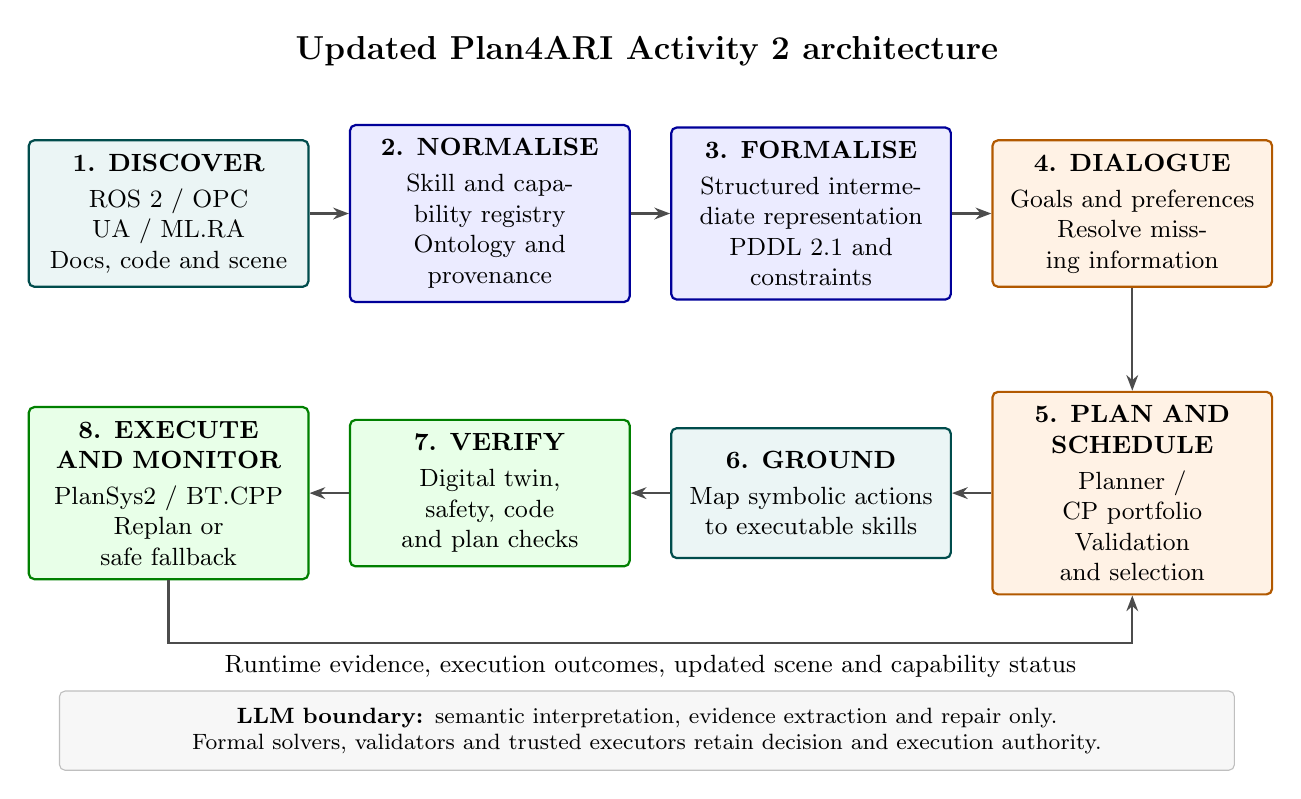
\begin{tikzpicture}[
  font=\sffamily,
  stage/.style={
    rounded corners=2pt,
    line width=.8pt,
    text width=3.2cm,
    minimum height=1.65cm,
    align=center,
    inner sep=5pt,
    font=\small
  },
  discover/.style={stage, draw=teal!60!black, fill=teal!8},
  model/.style={stage, draw=blue!60!black, fill=blue!8},
  dialogue/.style={stage, draw=orange!70!black, fill=orange!10},
  execution/.style={stage, draw=green!50!black, fill=green!9},
  flow/.style={-{Stealth[length=2mm]}, draw=black!70, line width=.8pt},
  node distance=8mm and 5mm
]

\node[font=\bfseries\large, align=center] (title) at (0,0)
  {Updated Plan4ARI Activity 2 architecture};

\node[discover, below=8mm of title, xshift=-6.075cm] (step1)
  {\textbf{1. DISCOVER}\\[2pt]
   ROS 2 / OPC UA / ML.RA\\Docs, code and scene};
\node[model, right=of step1] (step2)
  {\textbf{2. NORMALISE}\\[2pt]
   Skill and capability registry\\Ontology and provenance};
\node[model, right=of step2] (step3)
  {\textbf{3. FORMALISE}\\[2pt]
   Structured intermediate representation\\PDDL 2.1 and constraints};
\node[dialogue, right=of step3] (step4)
  {\textbf{4. DIALOGUE}\\[2pt]
   Goals and preferences\\Resolve missing information};

\node[execution, below=15mm of step1] (step8)
  {\textbf{8. EXECUTE AND MONITOR}\\[2pt]
   PlanSys2 / BT.CPP\\Replan or safe fallback};
\node[execution, right=of step8] (step7)
  {\textbf{7. VERIFY}\\[2pt]
   Digital twin, safety, code\\and plan checks};
\node[discover, right=of step7] (step6)
  {\textbf{6. GROUND}\\[2pt]
   Map symbolic actions\\to executable skills};
\node[dialogue, right=of step6] (step5)
  {\textbf{5. PLAN AND SCHEDULE}\\[2pt]
   Planner / CP portfolio\\Validation and selection};

\draw[flow] (step1.east) -- (step2.west);
\draw[flow] (step2.east) -- (step3.west);
\draw[flow] (step3.east) -- (step4.west);
\draw[flow] (step4.south) -- (step5.north);
\draw[flow] (step5.west) -- (step6.east);
\draw[flow] (step6.west) -- (step7.east);
\draw[flow] (step7.west) -- (step8.east);

\coordinate (feedback-path) at ($(step8.south)+(0,-8mm)$);
\draw[flow] (step8.south) -- (feedback-path) -| (step5.south);
\node[font=\small, fill=white, inner sep=2pt, align=center]
  at ($(step8.south)!0.5!(step5.south)+(0,-10mm)$)
  {Runtime evidence, execution outcomes, updated scene and capability status};

\node[draw=black!25, fill=black!3, rounded corners=2pt,
  text width=14.5cm, align=center, inner sep=6pt,
  font=\footnotesize, below=14mm of step8.south, xshift=6.075cm] (llm-boundary)
  {\textbf{LLM boundary:} semantic interpretation, evidence extraction and repair only.\\
   Formal solvers, validators and trusted executors retain decision and execution authority.};
\end{tikzpicture}
\caption{Updated end-to-end architecture for Activity~2, from controlled discovery to monitored execution.}\label{fig:architecture}
\end{figure}

\subsection{Stage 1~-~Controlled discovery}\label{sec:discovery}
Discovery is performed through authenticated tools with explicit read permissions. ROS\,2 discovery captures the computational graph and message/service/action definitions. PlanSys2 and MI.RA/Dexter adapters enumerate registered action executors and low-code blocks. Industrial adapters inspect authorized OPC UA methods and variables, PLC metadata, AutomationML/AAS models, and configuration files. Retrieval tools index manuals, process specifications, package manifests, code, and test evidence. Perception provides the current scene graph and object state.

The output is evidence, not yet a capability. Each observation is timestamped and linked to its source. Conflicts are retained for resolution. The system must distinguish ``present on the network'', ``callable'', ``tested'', ``approved for planning'', and ``approved for execution''.

\subsection{Stage 2~-~Capability and skill registry}\label{sec:registry}
\begin{figure}[htbp]
  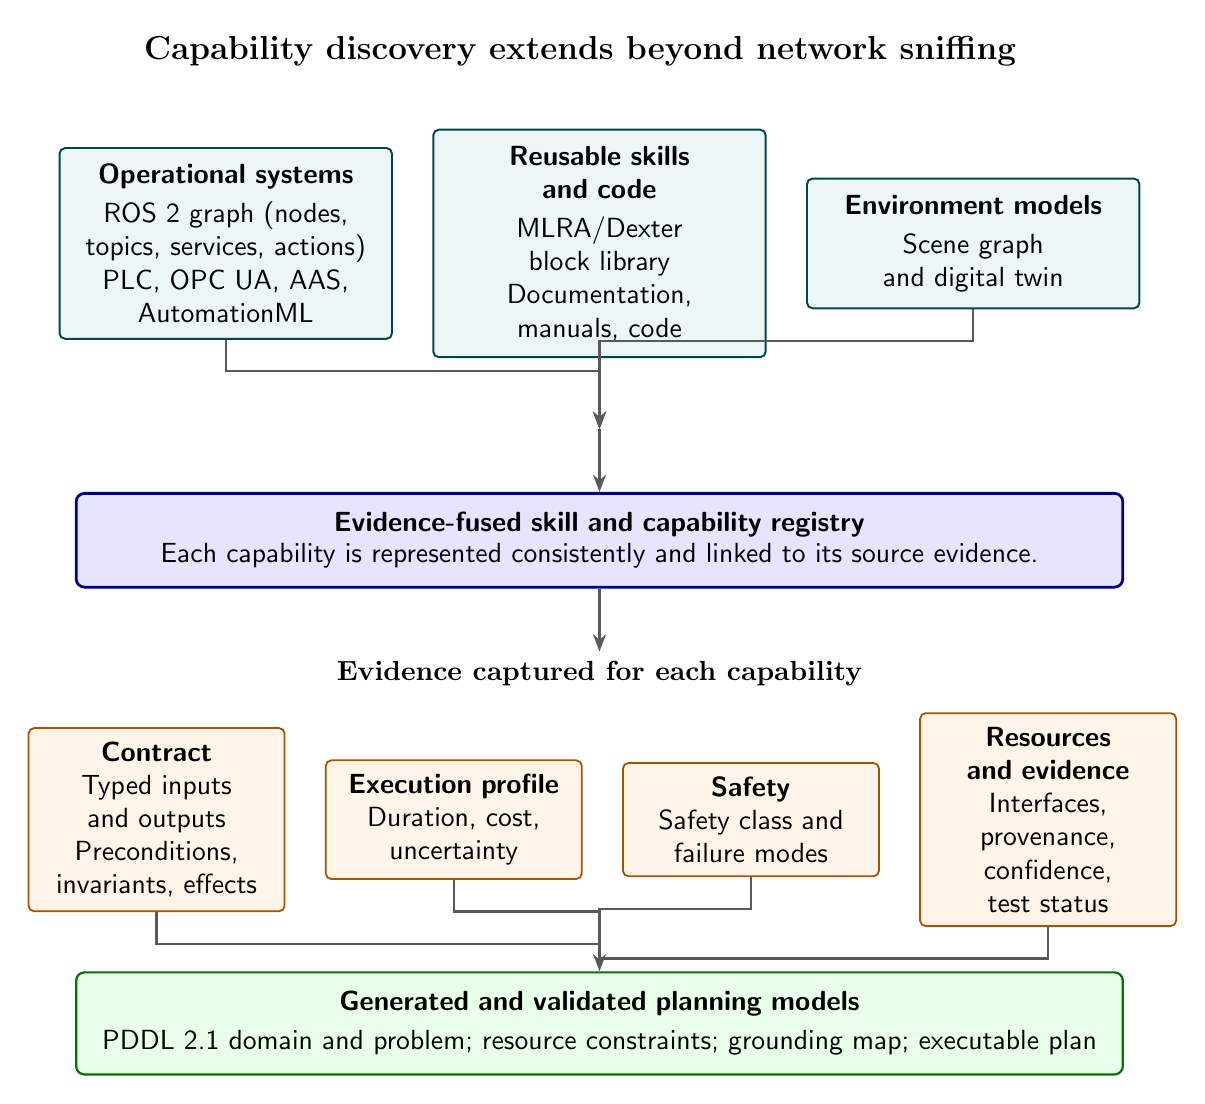
\begin{tikzpicture}[
  font=\sffamily,
  source/.style={
    draw=teal!55!black,
    fill=teal!7,
    rounded corners=2pt,
    line width=.7pt,
    text width=3.8cm,
    minimum height=1.55cm,
    align=center,
    inner sep=6pt
  },
  registry/.style={
    draw=blue!55!black,
    fill=blue!10,
    rounded corners=3pt,
    line width=1pt,
    text width=12.8cm,
    minimum height=1.05cm,
    align=center,
    inner sep=7pt
  },
  evidence/.style={
    draw=orange!65!black,
    fill=orange!9,
    rounded corners=2pt,
    line width=.65pt,
    text width=2.9cm,
    minimum height=1.15cm,
    align=center,
    inner sep=5pt
  },
  output/.style={
    draw=green!45!black,
    fill=green!9,
    rounded corners=3pt,
    line width=.8pt,
    text width=12.8cm,
    minimum height=1.15cm,
    align=center,
    inner sep=7pt
  },
  flow/.style={-{Stealth[length=2.2mm]}, draw=black!65, line width=.8pt},
  node distance=8mm and 5mm
]

\node[font=\bfseries\large, align=center] (title) at (0,0)
  {Capability discovery extends beyond network sniffing};

\node[source, below=9mm of title, xshift=-4.5cm] (operational)
  {\textbf{Operational systems}\\[2pt]
   ROS 2 graph (nodes, topics, services, actions)\\
   PLC, OPC UA, AAS, AutomationML};
\node[source, right=of operational] (skills)
  {\textbf{Reusable skills and code}\\[2pt]
   MLRA/Dexter block library\\
   Documentation, manuals, code};
\node[source, right=of skills] (environment)
  {\textbf{Environment models}\\[2pt]
   Scene graph and digital twin};

\coordinate (merge) at ($(skills.south)+(0,-9mm)$);
\draw[flow] (operational.south) -- ++(0,-4mm) -| (merge);
\draw[flow] (skills.south) -- (merge);
\draw[flow] (environment.south) -- ++(0,-4mm) -| (merge);

\node[registry, below=8mm of merge] (registry)
  {\textbf{Evidence-fused skill and capability registry}\\[-1pt]
   Each capability is represented consistently and linked to its source evidence.};
\draw[flow] (merge) -- (registry.north);

\node[font=\bfseries, below=8mm of registry] (evidence-title)
  {Evidence captured for each capability};
\node[evidence, below=4mm of evidence-title, xshift=-5.625cm] (contract)
  {\textbf{Contract}\\Typed inputs and outputs\\Preconditions, invariants, effects};
\node[evidence, right=of contract] (profile)
  {\textbf{Execution profile}\\Duration, cost, uncertainty};
\node[evidence, right=of profile] (safety)
  {\textbf{Safety}\\Safety class and failure modes};
\node[evidence, right=of safety] (evidence-data)
  {\textbf{Resources and evidence}\\Interfaces, provenance, confidence, test status};

\coordinate (out-merge) at ($(evidence-title.south)+(0,-27mm)$);
\draw[flow] (registry.south) -- (evidence-title.north);
\draw[draw=black!65, line width=.8pt] (contract.south) -- ++(0,-4mm) -| (out-merge);
\draw[draw=black!65, line width=.8pt] (profile.south) -- ++(0,-4mm) -| (out-merge);
\draw[draw=black!65, line width=.8pt] (safety.south) -- ++(0,-4mm) -| (out-merge);
\draw[draw=black!65, line width=.8pt] (evidence-data.south) -- ++(0,-4mm) -| (out-merge);

\node[output, below=8mm of out-merge] (planning)
  {\textbf{Generated and validated planning models}\\[2pt]
   PDDL 2.1 domain and problem; resource constraints; grounding map; executable plan};
\draw[flow] (out-merge) -- (planning.north);
\end{tikzpicture}
\caption{Multi-source discovery and the evidence-fused capability/skill registry.}\label{fig:registry}
\end{figure}

The registry is the stable semantic layer between the operational system and planning. A minimum skill record contains: unique identifier and version; provider and deployment endpoint; semantic description; typed inputs and outputs; preconditions, invariants and effects; required resources; interface binding; nominal and observed duration distributions; cost/quality models; safety class; failure modes and recovery options; effect-observation method; provenance and confidence; test status; and approval state.

\subsection{Stage 3~-~Formalisation through a typed intermediate representation}
The language model does not write final PDDL as its first artefact. It populates a schema-constrained intermediate representation using only types, predicates, resources and skills available from the registry, while clearly listing assumptions and missing information. A deterministic compiler converts the IR into PDDL~2.1, PDDL constraints, a CP model or another selected formalism. This separation simplifies validation, testing, migration and model comparison.

\subsection{Stage 4~-~Mixed-initiative user dialogue}
The dialogue component elicits goals, preferences, deadlines, quality criteria and acceptable trade-offs. It asks for human input only when the missing value cannot be derived from trusted sources or when alternatives have materially different safety, cost or process meaning. The user is shown a concise explanation of the interpreted goal, assumptions, unavailable capabilities and selected objective before planning.

\subsection{Stage 5~-~Hybrid planning and scheduling}
A feature analyser selects the planning route. Classical state-transition problems use a PDDL planner. Durative and preference-rich problems use temporal planners. Multi-agent allocation and resource scheduling use CP/CP-SAT, optionally connected to a symbolic plan skeleton. TAMP or MoveIt\,2 feasibility checks refine actions that require geometric validity. A portfolio returns candidate plans, diagnostics and objective values. The plan selector uses deterministic criteria; an LLM may explain trade-offs but does not override hard constraints.

\subsection{Stage 6~-~Grounding to execution}
For each grounded planning action, the grounding service resolves an approved skill implementation and binds symbolic arguments to ROS\,2 entities, MI.RA/Dexter parameters, tools, objects and resources. It checks current availability, interface compatibility, parameter ranges and required observations. If a suitable executor is missing, the system returns a capability gap. A code-generation workflow may propose an adapter or executor only when the necessary lower-level functions are already approved and the generated code is not safety critical.

\subsection{Stage 7~-~Verification and digital twin}
Before release, the system validates the domain/problem, planner output, and grounding map; checks temporal/resource consistency; simulates the workflow in the digital twin; tests generated adapters; estimates execution-time distributions; and verifies policy and safety constraints. Failed checks generate machine-readable diagnostics that are routed to the appropriate repair node. A repaired artefact must pass the complete validation chain again.

\subsection{Stage 8~-~Execution, monitoring and replanning}
The approved plan is transformed into the execution structure supported by PlanSys2, BehaviorTree.CPP and MI.RA/Dexter. Runtime monitoring compares expected and observed action effects, scene state, resource state and time windows. Small deviations are handled by a dispatch policy or an approved local recovery. A symbolic discrepancy triggers plan repair or replanning from the updated state. If no validated recovery exists, the system enters a safe state and requests human intervention.

\subsection{Code-generation assurance gate}\label{sec:codegate}
\begin{table}[htbp]
\centering\small
\caption{Code-generation assurance gates.}\label{tab:gates}
\begin{plangrid}{|L{4.0cm}|Y|}
\planheadrow \thead{Gate} & \thead{Required evidence} \\ \hline
G0~-~Proposal & Generated source, declared purpose, target interface and provenance. \\ \hline
G1~-~Static checks & Compilation, type checks, linting, security scanning, dependency allow-list and licence scan. \\ \hline
G2~-~Unit tests & Generated tests plus project-maintained interface and boundary tests. \\ \hline
G3~-~Simulation & Digital-twin execution, expected effects, timing limits and failure injection. \\ \hline
G4~-~Integration & ROS\,2/MI.RA/Dexter integration tests in an isolated test namespace. \\ \hline
G5~-~Review & Human engineering approval, traceability to requirement and change record. \\ \hline
G6~-~Release & Signed container/package, SBOM, version pinning and rollback plan. \\ \hline
G7~-~Operational approval & Explicit approval for the target cell; generated code cannot migrate automatically between cells. \\ \hline
\end{plangrid}
\end{table}

\subsection{Security architecture}
\begin{itemize}
\item Separate the LLM/tool network from safety-related control networks through the existing Open IPC/Core IPC boundary.
\item Use least-privilege service accounts and allow-listed discovery actions.
\item Treat documentation, ROS\,2 messages and user prompts as untrusted input; defend against prompt injection and malicious metadata.
\item Never expose arbitrary shell, package installation or network access to the model in the production path.
\item Log prompts, tool calls, retrieved evidence, model/version, artefact hashes, validations and approvals.
\item Sign deployable artefacts and support deterministic rollback.
\end{itemize}

\subsection{First running mockup at M12}\label{sec:mockup}
The M12 mockup implements the initial neuro-symbolic workflow described in~\cite[Sec.~2.1, Fig.~1 and Sec.~3]{sandrini2026proposal}. It starts from an available PDDL domain, a natural-language operator request, optional textual context and access to the running ROS\,2 system. The expected outputs are a validated problem, a selected symbolic plan and an execution-grounding map that connects planned actions to concrete PlanSys2/ROS\,2 behaviours. The demonstration will use the simplified single-robot pick-and-place scenario identified in~\cite{sandrini2026proposal}.

\runin{Operator interface and workflow.} The graphical interface described in~\cite[Fig.~4]{sandrini2026proposal} accepts task requests and optional context and presents execution feedback. The LangChain-based workflow maintains structured state containing the domain signature, request, context, ROS\,2 evidence, generated problem, validation diagnostics, planner outputs and grounding information. Deterministic nodes perform parsing, compilation, validation and planner invocation. LLM engines generate or repair structured content; tool-using LLM agents query the robotic system when required.

\runin{Problem generation and repair.} The workflow extracts the domain types, predicates, numeric fluents and action schemas. It resolves missing information through available ROS\,2 introspection tools or operator clarification. The problem generator produces JSON containing objects, initial facts, numeric values, goals, assumptions and unresolved information. A deterministic compiler generates PDDL. Unified Planning model checks and VAL-based plan validation, as applicable to the selected planning features, provide diagnostics to a bounded repair loop. The demonstration record will identify the checks actually implemented.

\runin{Planning and execution grounding.} A planner portfolio, accessed through Unified Planning and compatible engines such as POPF or OPTIC, generates candidate plans. The mockup will record the configured engines and the plan-selection criterion. Each selected action is matched to an available PlanSys2 executor or ROS\,2 skill; concrete arguments and missing execution information are retrieved before dispatch. The run log will distinguish formal plan validity from successful skill binding and observed execution.

\runin{Missing executors and controlled code generation.} The proposal describes an external code-generation service, accessed through a web-server interface, for synthesising a missing PlanSys2-compatible executor from available ROS\,2 interfaces. Where demonstrated, this branch will record the generated artefact and the checks performed before execution, in line with Section~\ref{sec:codegate}. Unsupported actions must be reported as capability gaps. The demonstration report will identify enabled branches and limitations rather than imply complete automatic skill synthesis.

\runin{Research extensions and maturity.} Research Goal~2 in~\cite{sandrini2026proposal} relaxes the available-domain assumption through ontology-based skill discovery and domain generation. Research Goal~3 studies scene graphs for mechanical assemblies, disassembly BT generation and execution monitoring. These directions belong to the wider A2 programme. Any prototype elements shown at M12 will be labelled by their actual implementation and validation status. Full multi-source discovery, multi-robot evaluation, temporal robustness and industrial MI.RA/Dexter integration remain subsequent development objectives.

\runin{M12 evidence package.} D2.1 will identify the versioned mockup release and execution environment, provide setup and demonstration instructions, record the input domain and operator requests, and retain generated JSON/PDDL, validation diagnostics, selected plans, action bindings and execution logs. A demonstration recording or live demonstration will accompany the technical description. Quantitative results will be added only after the corresponding experiments have been performed.

\subsection{Industrial input to mockup design}
The M12 mockup description should identify which requirements, constraints, examples or review findings originated from COMAU and how they affected the implementation. Section~\ref{sec:comau} provides the contribution matrix and evidence record for this attribution. Scientific method development, prototype implementation, industrial review and later MI.RA/Dexter integration must be recorded as distinct contributions. No first-year Dexter integration is claimed merely because the mockup is designed for subsequent integration.

% =====================================================================
\section{Method selection and decision rationale}\label{sec:selected}

\subsection{Selected baseline stack}
\begin{table}[htbp]
\centering\small
\caption{Selected baseline stack per layer.}\label{tab:stack}
\begin{plangrid}{|L{2.5cm}|Y|L{3.4cm}|Y|}
\planheadrow \thead{Layer} & \thead{Primary selection} & \thead{Fallback/comparator} & \thead{Rationale} \\ \hline
Knowledge representation & Ontology-backed skill registry plus relational world/scene state. & Relational database or knowledge graph with equivalent schema. & Planning must be grounded in executable, versioned capabilities rather than free text. \\ \hline
LLM workflow & Provider-neutral tool-using workflow with typed state and schema outputs. & Single-model pipeline for baseline comparison. & Reduces coupling and allows deterministic nodes around probabilistic calls. \\ \hline
Formalisation & Typed JSON/ontology IR $\rightarrow$ deterministic PDDL~2.1 compiler. & Direct PDDL generation as experimental baseline. & Separates semantics from syntax and enables robust validation. \\ \hline
Planning & Unified Planning portfolio with classical and temporal engines. & Direct engine integration. & Supports feature-based engine selection and reproducible comparison. \\ \hline
Scheduling & CP/CP-SAT for resources, allocation and time windows. & PDDL temporal planner when model fits. & Better fit for heterogeneous resources and industrial scheduling. \\ \hline
Validation & VAL + UP model checks + planner diagnostics. & Additional SMT/OMT checks. & Independent deterministic evidence is required. \\ \hline
Execution & PlanSys2 + BehaviorTree.CPP/ROS2 adapters. & MI.RA/Dexter-native workflow executor. & Open research stack and industrial target can be compared and integrated. \\ \hline
Temporal uncertainty & STN/STNU-based dispatch and monitoring. & Robust margins or stochastic planner for specific cases. & Keeps uncertainty handling explicit at execution time. \\ \hline
Digital twin & Verification, timing estimation, parameter calibration and regression testing. & Hardware-in-the-loop tests. & Simulation supports assurance but does not replace formal planning. \\ \hline
Code generation & Sandboxed adapter/executor synthesis with gated release. & Manual implementation. & Captures Code-as-Policy benefits without granting uncontrolled execution authority. \\ \hline
\end{plangrid}
\end{table}

\subsection{Planner-selection logic}
\begin{table}[htbp]
\centering\small
\caption{Planner-selection logic by problem feature.}\label{tab:plannerselection}
\begin{plangrid}{|L{6.0cm}|Y|}
\planheadrow \thead{Problem feature} & \thead{Preferred method} \\ \hline
Discrete deterministic actions, no durations & Classical PDDL planner. \\ \hline
Durative actions, concurrency, preferences & Temporal PDDL planner such as POPF/OPTIC where supported. \\ \hline
Heterogeneous agents, resource capacities, calendars, assignment & Constraint programming/CP-SAT, potentially using an LLM-generated task skeleton. \\ \hline
Geometric feasibility and manipulation & Task-and-motion planning/MoveIt\,2 feasibility service. \\ \hline
Uncontrollable action durations & Temporal plan plus STNU controllability/dispatch analysis. \\ \hline
Stochastic outcomes or partially observable state & Research branch using contingent/stochastic planning; do not force into deterministic PDDL. \\ \hline
Emergency runtime deviation & Approved recovery BT or bounded plan repair; safe stop if validation deadline cannot be met. \\ \hline
\end{plangrid}
\end{table}

\subsection{Research hypotheses}
\begin{table}[htbp]
\centering\small
\caption{Research hypotheses and their evaluation.}\label{tab:hypotheses}
\begin{plangrid}{|L{0.8cm}|Y|L{5.6cm}|}
\planheadrow \thead{ID} & \thead{Hypothesis} & \thead{Evaluation} \\ \hline
H1 & Evidence-fused capability discovery produces more executable planning domains than text-only domain generation. & Compare domain validity and action-grounding success across discovery ablations. \\ \hline
H2 & A typed IR plus deterministic compiler and validator loop outperforms direct PDDL generation for compact local models. & Measure valid-domain/problem rate, repair iterations, latency and model size. \\ \hline
H3 & Hybrid PDDL + CP scheduling improves feasibility and makespan for multi-agent industrial tasks compared with LLM-only and PDDL-only baselines. & Benchmark increasing resources, precedence, calendars and agent heterogeneity. \\ \hline
H4 & Scene-graph and capability-registry grounding reduces hallucinated objects/actions and improves replanning accuracy. & Compare raw visual/text context, scene graph only and combined operational graph. \\ \hline
H5 & Generated adapters can reduce integration effort without increasing operational risk when passed through the assurance gate. & Measure engineering time, defects, test coverage and blocked unsafe releases. \\ \hline
H6 & A model-agnostic architecture allows smaller local models to meet industrial requirements for most structured tasks. & Compare local and hosted models under fixed validators and the same benchmark. \\ \hline
\end{plangrid}
\end{table}

\subsection{Fallback strategy}
If automatic domain generation remains below acceptance thresholds, the project will retain a manually approved domain library and use LLMs only for problem generation and dialogue. If code generation does not pass the assurance gate reliably, missing skills will be implemented manually while the system still reports capability gaps. If PlanSys2 cannot support a required PDDL feature, the planning core will remain behind the Unified Planning abstraction and a custom executor adapter will translate the validated plan to MI.RA/Dexter/BehaviorTree.CPP.

% =====================================================================
\section{Benchmarking and validation plan}\label{sec:bench}

\subsection{Benchmark philosophy}
\begin{planbox}
Evaluation must cover the complete no-code chain. A system is not successful because it produces plausible text or valid PDDL syntax. It succeeds when the user's intent is represented correctly, the model is valid, the solver finds a feasible/optimal plan, each action is grounded, the plan executes under controlled perturbations and the process is faster for a process expert than the baseline programming method.
\end{planbox}

\subsection{Benchmark domains}
\begin{table}[htbp]
\centering\small
\caption{Benchmark domains.}\label{tab:domains}
\begin{plangrid}{|L{3.6cm}|Y|Y|}
\planheadrow \thead{Domain} & \thead{Core capabilities} & \thead{Planning challenges} \\ \hline
Single-arm pick and place & Object detection, grasp, move, place, I/O. & Grounding, missing objects, parameter binding and simple ordering. \\ \hline
Quality inspection & Camera setup, acquire, inspect, classify, report. & Conditional effects, information gathering and uncertain outcomes. \\ \hline
Welding process & Tool setup, seam selection, welding, inspection. & Durations, process constraints, no mid-seam replanning and safety stops. \\ \hline
Mechanical disassembly/ remanufacturing & Fastener/tool identification, grasping, removal and part handling. & Scene-graph precedence, accessibility, tool resources and effect validation. \\ \hline
Multi-robot material handling & Multiple arms/mobile manipulators and shared zones. & Allocation, scheduling, resource conflicts, travel time and makespan. \\ \hline
Human-robot collaborative assembly & Human and robot skills, shared resources and safety zones. & Uncertain human durations, task allocation, safe coordination and replanning. \\ \hline
\end{plangrid}
\end{table}

\subsection{Dataset structure}
\begin{itemize}
\item At least 10 cell/domain contexts for capability and domain discovery, consistent with the original KB KPI.
\item At least 100 natural-language task requests for problem generation, with paraphrases, ambiguity and missing information.
\item At least 100 plan-generation cases spanning classical, temporal and resource-constrained problems.
\item At least 100 plan-to-execution cases with ground-truth skill mappings and parameter bindings.
\item Perturbation variants: missing node, unavailable tool, delayed action, changed object state, failed perception, resource conflict and operator intervention.
\item Versioned benchmark artefacts: registry snapshots, domains, problems, plans, validation logs, expected execution traces and expert judgements.
\end{itemize}

\subsection{Metrics and proposed thresholds}
{\small\renewcommand{\arraystretch}{1.25}
\begin{longtable}{|L{3.6cm}|L{6.0cm}|L{5.7cm}|}
\caption{Metrics and proposed acceptance thresholds.}\label{tab:metrics}\\ \hline
\planheadrow \thead{Metric} & \thead{Definition} & \thead{Proposed acceptance/target} \\ \hline\endfirsthead
\hline\planheadrow \thead{Metric} & \thead{Definition} & \thead{Proposed acceptance/target} \\ \hline\endhead
Capability discovery precision/recall & Correct discovered capabilities and required fields against expert registry. & Report per source and fused result; target $\geq 0.90$ F1 for approved capability classes. \\ \hline
Provenance completeness & Share of registry facts linked to source and confidence. & 100\% for facts used in released planning models. \\ \hline
Domain validity & Syntactic/semantic validation and ability to solve reference instances. & 100\% syntax; $\geq 90\%$ semantically correct before human repair; 100\% for released domains. \\ \hline
Problem validity & Typed objects, initial state and goal consistent with domain. & $\geq 95\%$ after automatic repair; 100\% before planning release. \\ \hline
Plan validity & Independent validator accepts the plan. & 100\% of executed plans. \\ \hline
Goal correctness & Plan achieves the interpreted user goal and constraints. & $\geq 95\%$ on benchmark; disagreements adjudicated by experts. \\ \hline
Grounding success & Actions mapped to approved executors with valid parameters. & $\geq 90\%$ without new code; 100\% before execution. \\ \hline
Optimality/schedule quality & Makespan/cost relative to optimum or best known baseline. & Report gap; no regression against selected solver baseline. \\ \hline
Programming-time reduction & Time from request to approved executable workflow versus current MI.RA/Dexter/manual process. & Maintain contractual 66\% target. \\ \hline
Non-expert usability & Task completion by process expert without robotics programming training. & Maintain contractual objective; measure success, workload and interventions. \\ \hline
Runtime robustness & Successful completion under defined perturbations. & Domain-specific threshold; zero unsafe continuation after invalid state. \\ \hline
Generated-code release rate & Candidate code passing all gates without manual correction. & Research metric; no minimum, zero bypasses of assurance gate. \\ \hline
Latency and compute & End-to-end and stage-level time, memory, GPU/CPU and model calls. & Meet task-specific interactive and replanning budgets. \\ \hline
Fleet scale & Supported agents and concurrent tasks. & 3 mobile manipulators or 4 industrial arms, consistent with baseline. \\ \hline
\end{longtable}}

\subsection{Baselines and ablations}
\begin{itemize}
\item Direct LLM plan generation.
\item Direct natural-language-to-PDDL generation.
\item Text-only domain generation versus ROS\,2-only, documentation-only, scene-only and fused discovery.
\item Single planner versus planner portfolio and PDDL-only versus PDDL+CP.
\item Scene graph versus raw perception summary versus combined operational knowledge graph.
\item Hosted frontier model versus local open-weight model under identical validators.
\item With and without human confirmation at ambiguity gates.
\item With and without digital-twin verification.
\end{itemize}

\subsection{Statistical treatment}
Report success proportions with confidence intervals, paired comparisons on the same tasks, medians and percentile latency, and bootstrap intervals for optimality/time differences. Separate model-generation variance from planner determinism by repeating probabilistic stages with fixed and varied seeds. Publish the exact model identifiers, prompts, schemas, tool versions and artefact hashes for each benchmark run.

\subsection{Mockup evaluation and evidence for the journal manuscript}\label{sec:mockupeval}
The initial evaluation follows~\cite[Sec.~3]{sandrini2026proposal}, starting with a simplified single-robot pick-and-place scenario. It will assess problem-generation validity, repair success, planning success, plan quality and execution-grounding success. Execution completion and observed effects will be recorded separately from planning success. Failure cases will include missing information, unavailable skills and unsuccessful grounding where supported by the implemented mockup.

The proposal reports preliminary use of Llama~3.1--8B up to symbolic plan generation and plans comparisons between open-weight and closed-source models. This revision does not introduce numerical results or claim a completed comparison. The manuscript will report the exact tested backends, versions, prompts, planner configuration, cases and computational environment, with repeated runs where needed to characterise model variability.

The manuscript evidence package will include the architecture, implemented scope, reproducible protocol, measured results, failure analysis and limitations. Initial prototype findings will be distinguished from the later A2-wide KPI campaign, including the 66\% programming-time reduction and target fleet scale. Journal submission will provide an additional dissemination output; the running mockup and its evidence remain part of the M12 D2.1 delivery.

% =====================================================================
\section{COMAU contributions to industrial design}\label{sec:comau}

This section structures the evidence for COMAU participation in the first-year design of Activity~2. The technical specification assigns the Host Institution a role in use-case development, interaction with the Research Organization and sharing simulation environments and tools. The material currently available does not establish which of the contributions below were performed, by whom or for how long. Each entry therefore remains subject to confirmation through project records.

\subsection{Reporting scope and evidence status}
Separate three categories: pre-existing technology and know-how; project-specific activities performed during the reporting period; and work planned for later phases. Record an activity as completed only when its contributor, period, output and supporting evidence can be identified. A design input may have substantial scientific value without implying a large volume of personnel effort. Financial effort is not estimated from this technical contribution matrix.

\subsection{Potential contributions and expected evidence}
The following matrix is a framework for collecting and assessing contributions. It is not a statement of completed work.

\begin{table}[htbp]
\centering\small
\caption{Potential COMAU contributions and expected evidence.}\label{tab:comau}
\begin{plangrid}{|L{3.6cm}|Y|Y|}
\planheadrow \thead{Potential COMAU contribution} & \thead{Effect on method and mockup} & \thead{Evidence to retrieve} \\ \hline
Dexter programming workflow analysis & Identify decisions that currently require specialist expertise and those suitable for automation. & Annotated demonstrations, example workflows, meeting notes and emails. \\ \hline
Block-library analysis & Specify how a block becomes a plannable skill: parameters, preconditions, effects, resources and errors. & Module descriptions, configuration examples and technical annotations. \\ \hline
Industrial requirements definition & Inform structured generation, validation and explicit handling of missing capabilities. & Requirements, architecture review comments and documented decisions. \\ \hline
Use-case definition & Define realistic process sequences, constraints, variants and mockup failure conditions. & Use-case specification, process examples and test scenarios. \\ \hline
Future interface design & Specify the mapping between symbolic actions, ROS\,2 skills and Dexter modules for subsequent integration. & Interface diagrams, preliminary mappings and compatibility assessments. \\ \hline
Mockup review and acceptance criteria & Assess industrial relevance and define how the usefulness of the prototype will be measured. & Demo feedback, annotated tests, issue lists and resulting corrections. \\ \hline
\end{plangrid}
\end{table}

\subsection{Contribution records}\label{sec:contribrecords}
Create one record per contribution confirmed by COMAU, using the fields below. Retain unresolved records as pending. A note prepared after the activity should state its preparation date and identify the earlier records used to reconstruct the contribution.

\begin{table}[htbp]
\centering\small
\caption{Fields of a contribution record.}\label{tab:records}
\begin{plangrid}{|L{4.2cm}|Y|}
\planheadrow \thead{Field} & \thead{Information to complete} \\ \hline
Record identifier and status & COMAU-A2-[number]; pending evidence, confirmed, or planned. \\ \hline
Contributor and period & Named contributor, team, date or reporting period, and role. \\ \hline
Input and source & Requirement, workflow, module description, review comment or simulation asset; exact source reference and date. \\ \hline
Design decision and attribution & Decision informed by the input, alternatives considered, and distinction between COMAU input, joint decisions and Research Organization development. \\ \hline
Mockup or method effect & Affected component, interface, experiment, code version or document section. \\ \hline
Verification and follow-up & Review result, unresolved issue, responsible person and completion status. \\ \hline
Effort record reference & Reference to applicable personnel records, if available. Do not infer hours from the contribution category or budget. \\ \hline
\end{plangrid}
\end{table}

\subsection{Design decisions to document}
\runin{Capability semantics.} Identify whether COMAU input defined module preconditions, effects, parameter constraints, failure conditions or success observations beyond the existing block interface. Link each confirmed input to the corresponding capability record or formal action model.

\runin{Use case and evaluation.} Identify whether COMAU supplied process sequences, realistic variants, operating constraints, baseline workflows or acceptance criteria. Link confirmed contributions to the M12 demonstration and the evaluation protocol in Section~\ref{sec:mockupeval}.

\runin{Architecture and integration preparation.} Identify whether COMAU reviewed the separation between planning, validation and execution, the mapping to Dexter modules, or compatibility with simulation and deployment environments. Record future integration actions separately from completed first-year design work.

\subsection{Contribution summary for the reporting period}
\begin{planbox}
To be completed after the contribution records have been reviewed: confirmed COMAU activities and outputs; their effect on research directions and mockup design; contribution boundaries relative to the Research Organization; outstanding evidence; and actions planned for the next period. The final summary should cite the record identifiers in Section~\ref{sec:contribrecords} and include only substantiated activities.
\end{planbox}

% =====================================================================
\section{Updated implementation roadmap}\label{sec:roadmap}

\subsection{M12 mockup and work breakdown M13--M36}
\begin{table}[htbp]
\centering\small
\caption{M12 mockup and work breakdown M13--M36 with decision gates.}\label{tab:roadmap}
\begin{plangrid}{|L{1.6cm}|Y|Y|}
\planheadrow \thead{Period} & \thead{Technical focus} & \thead{Main outputs/decision gate} \\ \hline
M12 & First running mockup based on the neuro-symbolic workflow in~\cite{sandrini2026proposal}. & D2.1 scientific plan, running mockup, demonstration and reproducibility evidence; Gate D0. \\ \hline
M13--M15 & Benchmark formalisation; capability ontology; discovery adapters for ROS\,2 and MI.RA/Dexter. & Registry schema v1; benchmark v1; decision on supported PDDL subset and planning API. \\ \hline
M16--M18 & Multi-source capability extraction; typed IR; deterministic PDDL compiler; validators. & Discovery MVP; NL-to-IR-to-PDDL prototype; Gate D1 on domain/problem validity. \\ \hline
M18--M21 & Planner portfolio, CP scheduling and action-grounding service. & Validated plan pipeline; skill matching; Gate D2 on plan validity and grounding. \\ \hline
M20--M24 & PlanSys2/BehaviorTree.CPP execution; temporal network and uncertain-duration monitoring. & Execution prototype; plan-to-BT mapping; Gate D3 on temporal and runtime behaviour. \\ \hline
M22--M27 & Digital-twin verification, timing/cost learning and selected TAMP integration. & Simulation verification pipeline; schedule-quality evidence; MCTS go/no-go for selected domains. \\ \hline
M25--M30 & Code-generation assurance workflow and MI.RA/Dexter integration. & Sandbox, tests, signed containers; integrated low-code workflow; Gate D4 on software assurance. \\ \hline
M28--M34 & Online state/effect monitoring, plan repair, replanning and approved recoveries. & Runtime monitoring and recovery library; Gate D5 on robustness and safety response. \\ \hline
M31--M36 & Industrialisation, fleet-scale evaluation, documentation and handover. & Benchmark report, KPI evidence, integration package and final Activity~2 technical baseline. \\ \hline
\end{plangrid}
\end{table}

\subsection{Mapping to contractual tasks}
\begin{table}[htbp]
\centering\small
\caption{Updated internal interpretation of the contractual tasks.}\label{tab:taskmapping}
\begin{plangrid}{|L{2.4cm}|Y|}
\planheadrow \thead{Contractual task} & \thead{Updated internal interpretation} \\ \hline
T2.2 & Capability and domain discovery; natural-language problem generation; typed IR; lightweight/local model benchmarking; deterministic PDDL compilation. \\ \hline
T2.3 & Validated temporal plan-to-execution transformation; BT generation from selected plans; STN/STNU dispatch and duration-uncertainty monitoring. \\ \hline
T2.4 & Hybrid planner/CP optimisation; digital-twin verification and timing/cost estimation; optional MCTS/TAMP research branches. \\ \hline
T2.5 & Grounded plan execution; expected-effect monitoring; bounded plan repair/replanning; approved recovery and safe fallback. \\ \hline
T2.6 & MI.RA/Dexter block discovery, workflow generation, containerised integration and industrial security assurance. \\ \hline
T2.7 & CI/CD, model and prompt versioning, test automation, SBOM, signing, reproducible benchmark and audit logs. \\ \hline
T2.8 & Benchmark governance, ground truth, end-user tests and ongoing regression evaluation. \\ \hline
\end{plangrid}
\end{table}

\subsection{Responsibilities}
\begin{table}[htbp]
\centering\small
\caption{Responsibilities per role/organisation.}\label{tab:responsibilities}
\begin{plangrid}{|L{3.8cm}|Y|}
\planheadrow \thead{Role/organisation} & \thead{Primary contribution} \\ \hline
PI/Activity lead & Scientific direction, decision gates, integration priorities, and acceptance of methodological changes. \\ \hline
CNR & Architecture, capability discovery, LLM workflows, robotics integration, code assurance, benchmarks, and prototypes. \\ \hline
CNR/planning specialists & Planning/scheduling formalisms, planner portfolio, temporal uncertainty, validation, and optimization methods. \\ \hline
COMAU/Host Institution & Industrial requirements, use-case definition, Dexter capability/interface input and mockup review; later integration and end-user evaluation. First-year contributions are to be documented in Section~\ref{sec:comau}. \\ \hline
Activity 3/4 teams & Scene/state interfaces, motion-feasibility services, safety-aware motion planning, and execution feedback. \\ \hline
Activity 6 team & Human oversight, usability, trust, workload and acceptance measures. \\ \hline
\end{plangrid}
\end{table}

\subsection{Decision gates}
\begin{itemize}
\item \textbf{D0 (M12):} deliver the first running mockup with the scientific plan, demonstration instructions, versioned artefacts and observed execution evidence. Record implemented functions and limitations separately from later research extensions.
\item \textbf{D1 (M18):} proceed with automatic domain generation only if released domains achieve 100\% formal validation and acceptable semantic correctness; otherwise, use approved domain templates.
\item \textbf{D2 (M21):} select PDDL-only or PDDL+CP architecture based on multi-agent benchmark feasibility and schedule quality.
\item \textbf{D3 (M24):} confirm PlanSys2/BT execution route and supported temporal-uncertainty method.
\item \textbf{D4 (M30):} permit generated adapters in integration only after zero gate bypasses and successful rollback tests.
\item \textbf{D5 (M34):} approve online replanning only for scenarios where state updates, validation and safety response meet deadline budgets.
\end{itemize}

\subsection{Scientific manuscript and submission target}
A manuscript describing the first running mockup is planned for submission within one month of the 23 September 2026 revision, by 23 October 2026. The candidate destinations are IEEE Transactions on Automation Science and Engineering (IEEE T-ASE) and IEEE Transactions on Industrial Informatics (IEEE TII); the team will select one venue for submission.

The manuscript will present the neuro-symbolic architecture, the implemented mockup, the initial evaluation protocol and measured experimental results. Preparation comprises consolidating the mockup and reproducibility materials, completing experiments and failure analysis, finalising the manuscript and obtaining co-author approval. These steps support the stated submission target and do not imply that the experiments or submission have already occurred.

At submission, the project will record the selected journal, manuscript title, author list, submission date and acknowledgement or manuscript identifier. Acceptance and publication will be recorded separately if they occur. The submission date is a calendar target; no equivalence with the project M12 date is assumed in this document.

% =====================================================================
\section{Risks, ethics and regulatory alignment}\label{sec:risks}

\subsection{Technical and operational risk register}
{\small\renewcommand{\arraystretch}{1.25}
\begin{longtable}{|L{3.3cm}|L{1.6cm}|L{6.0cm}|L{3.8cm}|}
\caption{Technical and operational risk register (likelihood/impact: L = low, M = medium, H = high).}\label{tab:risks}\\ \hline
\planheadrow \thead{Risk} & \thead{Likelihood/ impact} & \thead{Mitigation} & \thead{Indicator} \\ \hline\endfirsthead
\hline\planheadrow \thead{Risk} & \thead{Likelihood/ impact} & \thead{Mitigation} & \thead{Indicator} \\ \hline\endhead
Hallucinated capability or action semantics & M/H & Multi-source evidence, provenance, schema constraints, expert approval and executable tests. & Unsupported symbols; grounding failures; provenance gaps. \\ \hline
Incorrect PDDL domain/problem & M/H & Typed IR, deterministic compiler, VAL/UP checks, reference problems and repair loop. & Validation failures; unsolved reference instances. \\ \hline
Valid but non-executable plan & M/H & First-class grounding map, resource and parameter checks, digital-twin execution. & Ungrounded actions; runtime precondition failures. \\ \hline
Unsafe or malicious user instruction & M/H & Policy gate, role-based access, safety constraints, prompt sanity checks and human approval. & Rejected requests; attempted policy bypass. \\ \hline
Prompt injection through documents/network metadata & M/H & Treat retrieved content as data, source allow-list, instruction isolation and tool permission boundaries. & Unexpected tool calls; retrieval-policy violations. \\ \hline
Generated insecure code & M/H & Restricted targets, static/security analysis, dependency allow-list, tests, review, signing and rollback. & Gate failures; vulnerabilities; unsigned artefacts. \\ \hline
Model/provider drift & H/M & Provider abstraction, frozen benchmark, model cards, requalification and local fallback. & Regression at decision gate; changed API behaviour. \\ \hline
Planner/representation mismatch & M/M & Feature analyser, planner portfolio, explicit unsupported-feature errors. & Engine failures; semantic translation gaps. \\ \hline
Temporal uncertainty exceeds model & M/H & Observed duration distributions, STNU/robust margins, replanning and safe stop. & Missed windows; non-controllability. \\ \hline
Discovery exposes sensitive network data & M/H & Least privilege, no passive sniffing by default, network segmentation, data minimisation and logs. & Unauthorised endpoints; excessive data collection. \\ \hline
Over-reliance on simulation & M/M & Hardware-in-the-loop, staged commissioning and real execution evidence. & Simulation-to-real discrepancy. \\ \hline
Insufficient non-expert usability & M/M & Mixed-initiative dialogue, explanation, user-centred testing and interface simplification. & High intervention/workload; low task completion. \\ \hline
\end{longtable}}

\subsection{Human oversight and explainability}
The system should expose a concise decision record: interpreted goal; assumptions; capabilities selected; unavailable or inferred information; formal constraints; objective function; selected plan and alternatives; validation results; generated-code status; and reasons for replanning or refusal. Human confirmation is mandatory for new domain approval, new code release, safety-relevant ambiguity and changes that exceed the validated operating envelope.

\subsection{EU AI Act}
Regulation (EU) 2024/1689 establishes harmonised rules for AI systems~\cite{eu2024aiact}. The exact classification of each \PlanARI{} component depends on its intended purpose and integration into machinery. The project should nevertheless implement risk management, data and technical documentation, logging, transparency, human oversight, accuracy, robustness and cybersecurity by design. The D2.1 architecture supports these requirements through traceable evidence, independent validation, access control and explicit approval gates.

\subsection{Machinery and cybersecurity regulation}
Regulation (EU) 2023/1230 on machinery becomes the relevant machinery framework from January 2027, while Regulation (EU) 2024/2847 introduces horizontal cybersecurity requirements for products with digital elements~\cite{eu2024cra,eu2023machinery}. \PlanARI{} should therefore maintain a clear boundary between experimental AI modules and safety functions, protect update and deployment channels, manage vulnerabilities and dependencies, preserve technical documentation and support secure rollback. This deliverable is not a conformity assessment; legal classification and harmonised-standard mapping require specialist review.

\subsection{Data protection and confidentiality}
\begin{itemize}
\item Minimise collection of user speech, network metadata and production documents.
\item Define retention, access and lawful basis for personal data used in dialogue and evaluation.
\item Keep proprietary process data on-premise when required; use local models or approved enterprise endpoints.
\item Redact or isolate credentials, personal data and trade secrets from model context and logs.
\item Document training/fine-tuning datasets and prevent unauthorised reuse of customer data.
\end{itemize}

\subsection{Research ethics}
Experiments involving workers must use informed consent, appropriate ethics review, data minimisation and separation between research evaluation and employment assessment. The no-code interface must not create a misleading impression that the robot understands more than it does. Uncertainty, assumptions, unavailable capabilities and reasons for refusal should be communicated clearly.

% =====================================================================
\section{Conclusions and proposed updates}\label{sec:conclusions}

\subsection{Final scientific position}
\begin{planbox}
The original \PlanARI{} objective remains timely. The most credible 2026 research position is not to make an LLM the planner, but to make it the semantic and knowledge-engineering layer of a verified planning system. Formal solvers, validators, explicit capability models and trusted executors provide determinism and industrial control. The resulting architecture is neuro-symbolic, capability-aware and model agnostic.
\end{planbox}

The restructuring proposal is therefore recommended, with two refinements. First, capability discovery must be broader and more controlled than ROS\,2 network sniffing: it requires semantic fusion across runtime interfaces, engineering data, documentation, code and scene state. Second, Code as Policies should be adopted as an inspiration for composing APIs and generating adapters, not as permission for unrestricted policy code to control industrial equipment.

\subsection{Proposed approval decisions}
\begin{enumerate}
\item Approve operational capability discovery and skill registry as the central research contribution of Activity~2.
\item Approve the NL-to-IR-to-PDDL formalization pipeline and independent validator/solver repair loop.
\item Approve a hybrid planner portfolio including classical/temporal planning and constraint programming.
\item Approve PlanSys2 and BehaviorTree.CPP as reference open execution technologies, subject to feature and integration validation.
\item Approve STN/STNU methods as temporal-dispatch and uncertainty-monitoring components.
\item Approve digital-twin verification and timing/cost estimation; retain MCTS as a domain-dependent research option rather than the baseline optimiser.
\item Approve gated code generation for symbolic solvers, adapters and candidate action executors; prohibit direct deployment or safety-critical generation.
\item Approve the revised benchmark and KPI framework while preserving the contractual high-level targets.
\item Approve the M12 mockup evidence package and the updated M13--M36 development roadmap and decision gates.
\item Place model families, VLA/world-action models and fully automatic domain generation on a monitored technology watch list.
\item Confirm the manuscript submission target of 23 October 2026 to one selected journal, IEEE T-ASE or IEEE TII, while recording acceptance and publication separately.
\end{enumerate}

\subsection{Open research questions}
\begin{itemize}
\item How much semantic capability information can be inferred reliably from a running ROS\,2 graph without manually authored annotations?
\item How should conflicting evidence from code, documentation, runtime behaviour and vendor metadata be reconciled?
\item Which skill ontology provides sufficient expressiveness without making domain generation too complex?
\item When should scheduling be compiled into PDDL, solved in CP, or handled by a coupled planner?
\item Can operational duration distributions be learned online while preserving temporal controllability and safety?
\item What is the minimum assurance evidence required for generated adapters in an industrial low-code platform?
\item How do scene-graph uncertainty and capability uncertainty propagate into plan selection and explanations?
\item How should user preferences and trust measures influence optimisation without weakening safety constraints?
\end{itemize}

\clearpage
% Sources listed in the Word version but not cited in the text ([R15]-[R17], [R26], [R40], [R41])
\nocite{singh2023progprompt,ahn2023saycan,lin2023text2motion,izzo2024btgenbot,colledanchise2018bt,btcpp_docs}
\bibliographystyle{IEEEtran}
\bibliography{references}
\end{document}
